\chapter{Quantum no-cloning theorem and cryptography}
\section{Quantum no-cloning theorem}
\subsection{Indistinguabilité des états non-orthogonaux}
\retenir{Les états quantiques non-orthogonaux ne sont pas parfaitement distinguables.}\ \\

En effets, des bits classiques sont, \textit{en principe}, complètement distinguables
\begin{equation}
\langle0|1\rangle =(0\ 1)\left(\begin{array}{c}
0\\
1
\end{array}\right) = 0
\end{equation}
Mais pour les qubits
\begin{equation}
\bra{\phi}\ket{\psi} \equiv (\gamma^*\ \delta^*)\left(\begin{array}{c}
\alpha\\
\beta
\end{array}\right) = \alpha\gamma^*+\beta\gamma^*\neq0
\end{equation}
où $\ket\psi \equiv \alpha\ket0+\beta\ket1$ et $\ket\phi\equiv\gamma\ket0+\delta\ket1$. Dès lors,
lorsqu'ils ne sont \textbf{pas} orthogonaux, ils sont \textit{intrinsèquement indistinguables}. Ceci
a plusieurs applications : codages quantiques, "quantum money", principe de non-clonage quantique, \dots

\subsubsection{Quantum coding (compression of quantum info)}
	\begin{wrapfigure}[5]{r}{5cm}
%	\vspace{-5mm}
	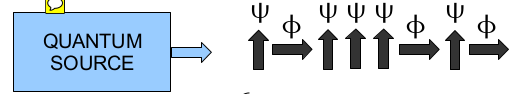
\includegraphics[scale=0.25]{ch3/image1}
	\captionof{figure}{ }
	\end{wrapfigure}
Soit une source qui émets une séquence de qubits identiquement distribué (probabilité $1/2$)
\begin{equation}
\left\{\begin{array}{lll}
\ket\psi &p=1/2&\ket\psi =\ket0\\
\ket\phi &p=1/2&\ket\phi =(\ket0+\ket1)/\sqrt{2}
\end{array}\right.
\end{equation}
Il s'agit d'un mélange d'états \textbf{non-orthogonaux} et donc indistinguables (produit scalaire entre
les deux de $1/\sqrt{2}$). Il n'est pas
possible de compresser une séquence de bits identiquement distribué, mais avec les qubits c'est
possible. En effet, $\ket\psi=\ket0$ mais $\ket\phi$ est une combinaison linéaire de 
$\ket1$ et $\ket2$ : c'est une superposition quantique qui n'a pas d'équivalent classique.\\

Calculons l'opérateur densité moyen. Il est nécessaire de la diagonaliser pour appliquer l'entropie
de \textsc{von Neumann} (qui est l'entropie de \textsc{Shannon} des valeurs propres)
\begin{equation}
\rho = \frac{1}{2}\left(\begin{array}{cc}
1&0\\
0&0
\end{array}\right)+\frac{1}{2}\left(\begin{array}{cc}
1/2&1/2\\
1/2&1/2
\end{array}\right)=\left(\begin{array}{cc}
3/4&1/4\\
1/7&1/4
\end{array}\right)\quad\Rightarrow\quad\left(\begin{array}{cc}
0.85&0\\
0&0.85
\end{array}\right)
\end{equation}
L'entropie de \textsc{von Neumann} vaut alors
\begin{equation}
S(\rho) = -\text{Tr}[\rho\log(\rho)] = 0.6 < 1\text{ bit}
\end{equation}
Celle-ci est inférieur à 1 bit, on peut donc faire une compression même avec $p=1/2$. C'est la \textbf{redondance
quantique}. Classiquement, ce n'est pas compressible mais le fait qu'ils soient indistinguables 
et que c'est un mélange, cela donne la possibilité de faire mieux. C'est le mélange qui a introduit
la redondance.

\subsubsection{Théorème de non-clonage quantique}
On aimerait avoir
\begin{equation}
\left\{\begin{array}{ll}
\ket\psi &= \alpha\ket0+\beta\ket1\\
\ket0
\end{array}\right.\qquad\Rightarrow\qquad\left\{\begin{array}{ll}
\ket\psi &= \alpha\ket0+\beta\ket1\\
\ket\psi &= \alpha\ket0+\beta\ket1\\
\end{array}\right.
\end{equation}
où $\ket0$ est l'état sur lequel on veut faire la copie ("page blanche"). On peut montrer que
ceci est \textbf{interdit par la physique}. C'est une conséquence du fait que deux états 
non-orthogonaux ne sont pas distinguables.


\subsubsection{Quantum money}
Si on attribue un numéro de série qui est une séquence de spin $1/2$ provenant d'atomes 
isolés dans des états non-orthogonaux, on ne serait pas habilité à lire ni cloner le billet.

\subsubsection{Cryptographie quantique (QKD)}
Il s'agit d'un des protocoles les plus connu (distribution de clef). Il y a deux parties 
autorisées ($A,B$) et un espion $E$. Grâce au théorème de non-clonage quantique, on peut
assurer la sécurité de la ligne malgré qu'elle soit "écoutée". Ce genre de dispositif est
déjà commercialisé (pour les communications par fibre optique sur 50 km).

\subsection{Optical qubits}
On reprends l'interféromètre du premier chapitre. Lire \textit{slides 8-15}, brièvement 
résumé ici.

\begin{itemize}
\item[$\bullet$] \textit{Interféromètre à un photon, $\theta=0$}. Si pas de lame de phase,
c'est toujours le même détecteur qui va cliquer. L'état du photon est dans une superposition
des deux chemins.
\item[$\bullet$] \textit{Interféromètre à un photon, $\theta=\pi$}. Si l'on place une
lame de phase de $\pi$ on a toujours que un seul clic, mais dans l'autre détecteur.
\item[$\bullet$] \textit{Interféromètre à un photon, $\theta=\pi/2$}. Si l'on place une
lame de phase de $\pi/2$. Classiquement, cela correspond à une intensité $50/50$ sur chaque détecteur. 
En quantique, on aura maximum un clic : "\textit{quantum randomness}". Il va y avoir un clic
sur le premier ou le deuxième détecteur, avec une probabilité de 50\% : c'est bien aléatoire. Ce
n'est pas un manque de connaissance, mais du à la nature même de la mécanique quantique.
\end{itemize}

	\begin{wrapfigure}[5]{r}{5cm}
	\vspace{-5mm}
	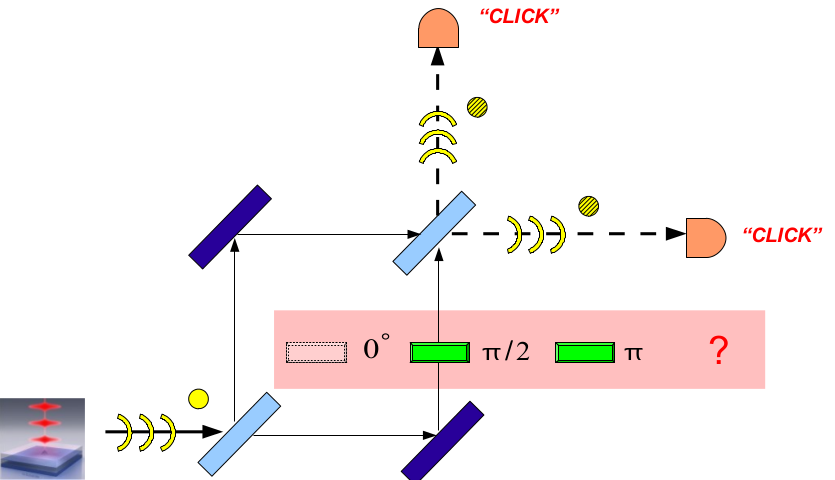
\includegraphics[scale=0.2]{ch3/image2}
	\captionof{figure}{ }
	\end{wrapfigure}
Il est donc \textbf{impossible de déterminer la lame de phase} insérée à partir de la connaissance
du détecteur qui a cliquer. L'espion sera dans cette situation : il voit quelque chose, mais ne 
sait pas la situation dans laquelle on se trouve.\\

	\begin{wrapfigure}[5]{r}{5cm}
%	\vspace{-5mm}
	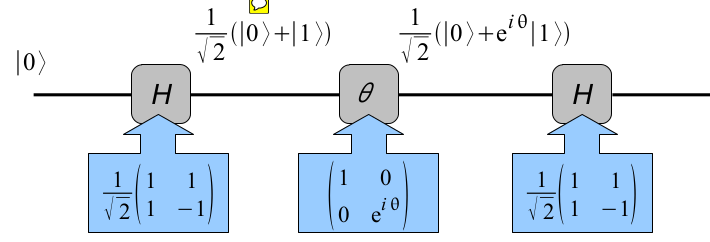
\includegraphics[scale=0.2]{ch3/image3}
	\captionof{figure}{ }
	\end{wrapfigure}
On peut ré-écrire les précédentes équations (chapitre 1), mais en présence d'une lame de phase.
La superposition entre les deux BS s'écrit cette fois-ci
\begin{equation}
\frac{1}{\sqrt{2}}\left(\ket0+e^{i\theta}\ket1\right)
\end{equation}
Avec les portes d'\textsc{Hadamard}, ré-écrivons notre circuit

\begin{equation}
H\ket0 = \frac{1}{\sqrt{2}}\left(\begin{array}{cc}
1&1\\
1&-1
\end{array}\right)\left(\begin{array}{c}
1\\
0
\end{array}\right)=\frac{1}{\sqrt{2}}\left(\begin{array}{c}
1\\
1
\end{array}\right) = \frac{1}{\sqrt{2}}(\ket0+\ket1)
\end{equation}
Appliquons la porte "quantum phase"
\begin{equation}
\Phi\left[\frac{1}{\sqrt{2}}(\ket0+\ket1)\right]=\left(\begin{array}{cc}
1&0\\
0&e^{i\theta}
\end{array}\right)\frac{1}{\sqrt{2}}\left(\begin{array}{c}
1\\
1
\end{array}\right)=\frac{1}{\sqrt{2}}\left(\begin{array}{c}
1\\
e^{i\theta}
\end{array}\right)=\frac{1}{\sqrt{2}}(\ket0+e^{i\theta}\ket1)
\end{equation}


	\begin{wrapfigure}[5]{r}{3.5cm}
	\vspace{-8mm}
	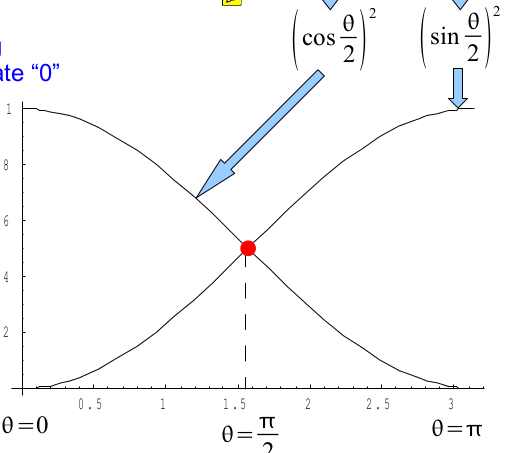
\includegraphics[scale=0.2]{ch3/image4}
	\captionof{figure}{ }
	\end{wrapfigure}
En appliquant une nouvelle fois \textsc{Hadamard}, on trouve finalement l'état de sortie\\	
\cadre{\begin{equation}
\dfrac{1+e^{i\theta}}{2}\ket0+\dfrac{1-{i\theta}}{2}\ket1
\end{equation}}\ 

La probabilité de mesurer $\ket0$ est donnée par $\left|\frac{1+e^{i\theta}}{2} \right|^2 = \cos^2\frac{\theta}{2}$ et la probabilité de mesurer $\ket1$ est de $\sin^2\frac{\theta}{2}$.\\

Mais qu'est ce que ceci vient faire pour le théorème de non-clonage quantique ? Il va nous montrer
pourquoi le clonage est interdit. L'origine de ce principe est la linéarité de la mécanique
quantique. Donnons nous deux bases 
\begin{description}
\item[Computational basis] $\{\ket0,\ket1\}$ (convention)
\item[Dual basis] $\ket\pm = (\ket0\pm\ket1)/\sqrt{2}$
\end{description}
Supposons que les états $\{\ket0,\ket1\}$ puissent être clonés
\begin{equation}
\begin{array}{ll}
\ket0 &\to \ket0\ket0\\
\ket1 &\to \ket1\ket1
\end{array}
\end{equation}
Si c'est le cas, les états $\{\ket+,\ket-\}$ ne peuvent pas l'être
\begin{equation}
\ket0+\ket1 \to \ket0\ket0+\ket1\ket1 \neq (\ket0+\ket1)(\ket0+\ket1)
\end{equation}
La première égalité est un état intriqué (état de \textsc{Bell}, $\ket Phi^+$), ce n'est pas ce
qu'on voulait car nous voulions le produit (seconde (non-)égalité). \textbf{Donc}
\begin{equation}
\ket\pm \nrightarrow \ket\pm\ket\pm
\end{equation}
Si on peut cloner l'un, on ne peut pas cloner l'autre. Le choix de la base étant arbitraire, on
comprend l'origine du théorème.

\newpage
\subsubsection{Exemple : qubit optique}
	\begin{wrapfigure}[5]{l}{8cm}
	\vspace{-5mm}
	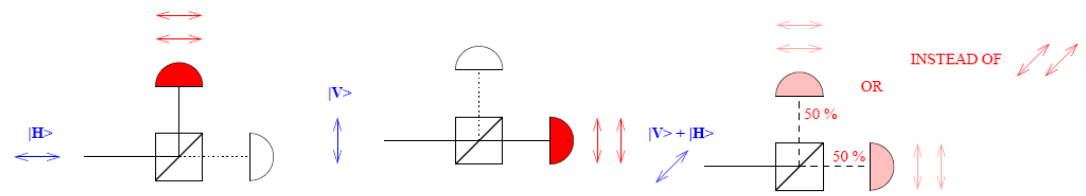
\includegraphics[scale=0.2]{ch3/image5}
	\captionof{figure}{ }
	\end{wrapfigure}
On a deux photons identiques dans la même polarisation. Si l'on vient avec $\ket V$, les deux
photons vont sortir du même côté et inversement avec $\ket H$. Si par contre on vient avec
$\ket V+\ket H$, on n'aura pas deux fois $\ket V+\ket H$ en sortie mais l'un des résultats
précédents avec une probabilité de 50\%.\\

On pourrait croire que l'amplification optique par émission stimulée viole le théorème. Mais 
l'émission stimulée s'accompagne toujours d'émission spontanée : les polarisation ne seront
dès lors pas indépendantes et le théorème ne sera pas violé.


\subsubsection{Causalité}
On peut montrer que si le clonage était possible, la causalité serait violée. Créons un état
de \textsc{Bell} $\ket{\Psi^-}$. On envoie un des qbits de cet état à gauche, l'autre à droite. 
A gauche, on va le mesurer dans la base de référence ou dans la base duale. Je peux ainsi calculer
les deux opérateurs densité : l'un dans la base de référence $\rho$ et l'autre dans la base
duale $\rho'$. Le problème c'est que $\rho\neq\rho'$ est \textbf{distinguable}. En effet, en mesurant
l'original et le clone, on sait que c'est plus probable d'avoir $\rho$ ou $\rho'$. En effectuant
la mesure, on a un état cloné. Si on peut dire lequel, on peut transmettre instantanément l'information
ce qui viole la causalité.\\

On peut montrer que le "meilleur" clonage possible correspond à une fidélité de $5/6$ : on peut
presque bien cloner, mais pas parfaitement. 


\section{Quantum cryptography}
Avec des bits classiques, Eve peut écouter ce qui se passe sur la ligne entre $A$ et $B$. Comment
être sur de la confidentialité ? C'est très simple, on utilise une clef secrète. Alice a le message, 
elle y ajoute une clef pour donner un \textit{cipher} puis envoie ce dernier à Bob. Si Bob à la clef,
il peut retrouver le message. C'est parfait, mais une clef ne peut pas être utilisée deux fois sinon
on perd la sécurité. Il existe d'autres techniques, comme avec la clef publique $E$ pour l'encodage
et une clef privée $D$ pour le décodage. C'est difficile de décoler l'information car déduire $D$ et
$E$ nécessite une factorisation ce qui est un "calcul difficile". Le problème c'est que un ordinateur
quantique sait faire ça efficacement (temps polynomial), ce qui rendrait le protocole non sécurisé.\\

Il existe une solution quantique, le protocole BB84. Dans ce protocole, l'encodage est classique
mais la distribution de la clef est quantique. On peut prouver que c'est sécurisé si
\begin{itemize}
\item[$\bullet$] La clef secrète est générée totalement aléatoirement. Si pseudo-aléatoire ça devient
prédictible et c'est foutu.
\item[$\bullet$] La clef secrète doit être aussi longue que le message.
\item[$\bullet$] La même clef secrète ne peut pas être utilisée pour différents messages.
\end{itemize}\ 

	\begin{wrapfigure}[5]{l}{6cm}
	\vspace{-5mm}
	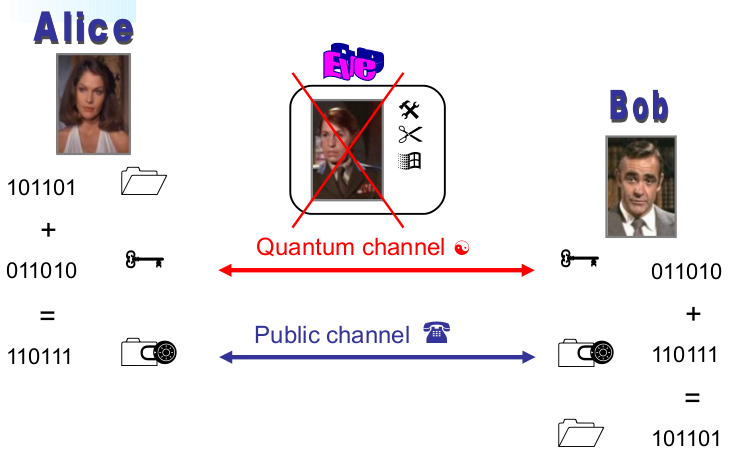
\includegraphics[scale=0.2]{ch3/image6}
	\captionof{figure}{ }
	\end{wrapfigure}
Ce qui est intéressant c'est que la \textbf{clef secrète} est \textbf{inconnue de Eve} : c'est
garanti par la mécanique quantique! Si Eve essaye d’espionner, cela va causer des erreurs de 
transmission ! S'il n'y a pas d'erreur, c'est que personne n'a essayé d’espionner. Avec la base
de codage, Alice code son signal et l'envoie à Bob. 

\newpage
	\begin{wrapfigure}[11]{l}{6cm}
	%\vspace{-5mm}
	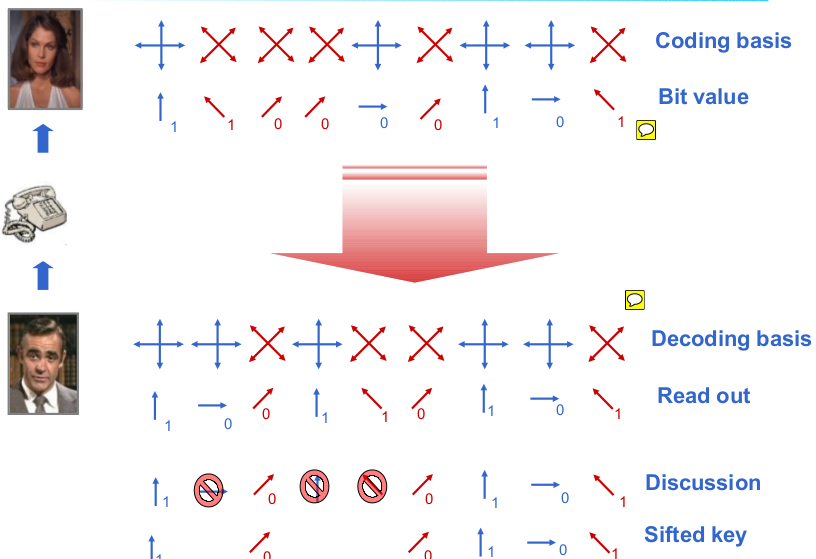
\includegraphics[scale=0.2]{ch3/image7}
	\captionof{figure}{ }
	\end{wrapfigure}
Le protocole BB84 nécessite l'utilisation de deux bases conjuguées. Alice a à sa disposition la
base de codage, composée de quatre états non-orthogonaux. Supposons pour le moment que la ligne
est parfaite, personne n'écoute.\\

Bob reçoit le bit codé. Il va prendre une base \textbf{aléatoire} pour décoder le signal, puis il
va essayer de distinguer horizontal, vertical, diagonal ou anti-diagonal. Évidemment, en faisant ça,
beaucoup sont faux. Vient ensuite une étape de discussion ou Alice et Bob vont parler des bases
utilisées et voir directement ce qui est faux. On obtient alors une \textbf{shifted key} : elle est
plus petite que la clef, mais elle est parfaite. Regardons maintenant s'il y a un espion.\\

	\begin{wrapfigure}[11]{r}{6cm}
	\vspace{-5mm}
	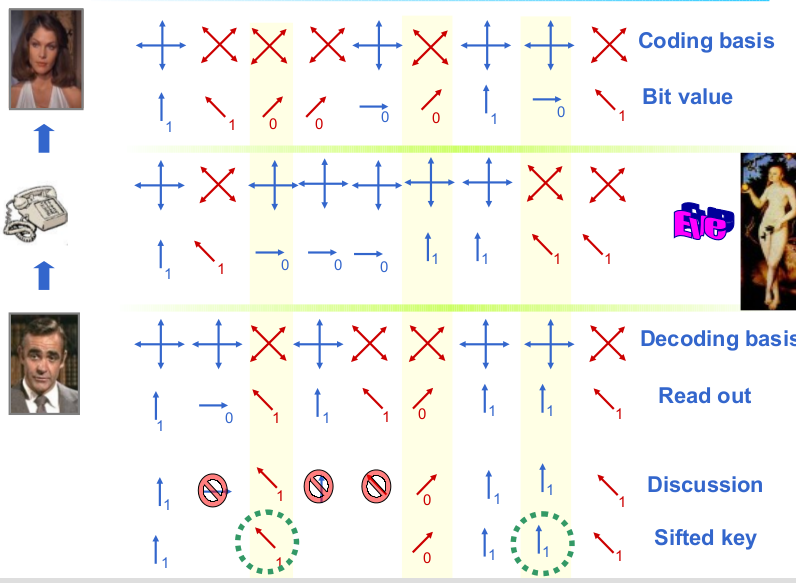
\includegraphics[scale=0.2]{ch3/image8}
	\captionof{figure}{ }
	\end{wrapfigure}
Cette fois-ci, Eve est entre les deux. Elle va essayer de faire comme Bob et choisir une base
au hasard. Elle va décoder avec et envoyer le résultat à Bob en espérant que ce soit exact. 
Bob choisi une base au hasard et essaye de décoder. Dans la première colonne, l'action de Eve
est invisible car elle a choisie la bonne base et Bob aussi. Dans la deuxième, c'est trouvé 
par Eve mais Bob a aussi choisi la mauvaise base. Vient ensuite la troisième
colonne : Alice à envoyé un 0, Eve utilise la mauvaise base ($H/V$) et envoie un $H$ à Bob. Bob
utilise la bonne base, mais $E$ l'a modifié : cela cause une erreur, entourée en vert. Ainsi,
dans les six bits de la shifted key, deux sont faux.\\

Nous allons voir que l'interception d'Eve est limitée par la physique quantique. En effet, Eve
doit faire une mesure sans savoir la base utilisée par Alice. Elle doit intercepter/renvoyer
avec la base $+$ ou $\times$, garder une copie de son coté, faire des mesures qui ne démolissent
pas l'état quantique, \dots Toutes ces opérations vont causer des erreurs de transmission : plus
Eve en sait, plus il y a d'erreurs. \\

	\begin{wrapfigure}[9]{l}{6cm}
	\vspace{-5mm}
	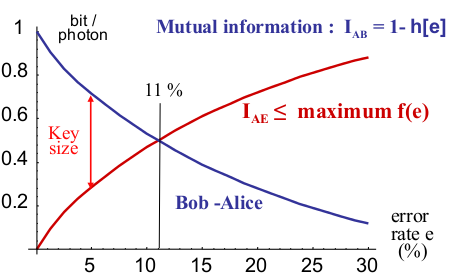
\includegraphics[scale=0.35]{ch3/image9}
	\captionof{figure}{ }
	\end{wrapfigure}
Analysons la pire situation, soit celle ou Eve applique la meilleur stratégie autorisée par la
mécanique quantique (courbe rouge). Il y a une intersection avec le taux d'erreur autour de 
11\% : tant que l'on est en dessous d'un taux d'erreur de 11\%, Bob en sait plus que Eve, il a
un avantage. En pratique, il existe un algorithme qui permet d'extraire une clef basé sur la
différence entre le taux d'erreur ce ce que sait Eve tant que l'on a un avantage. Dès lors, tant
que le rouge est en dessous de 11\%, on peut extraire une clef totalement secrète garantie par
la mécanique quantique.

\subsubsection{Procédure réelle}

\begin{center}
	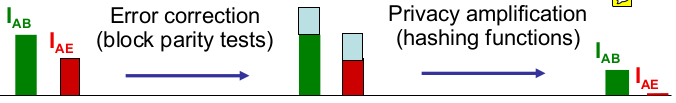
\includegraphics[scale=0.3]{ch3/image10}
	\captionof{figure}{ }
\end{center}

Après l'échange initial entre Alice et Bob, ils mesurent le taux d'erreur en comparant publiquement une petite partie de la clé brute. Ceci permet d'évaluer le montant de l'information que Eve a 
(possiblement) à disposition. Ensuite (et seulement si Bob en sait plus que Eve, soit si 
$QBER<0.11$) on applique une correction d'erreur et une amplification privée : $A$ et $B$ extraient
la clef disponible en corrigeant les erreurs et en annulant quasiment toute l'information que $E$ 
avait. Un premier setup mettant ça en application a été proposé par \textit{ID Quantique}.


\subsection{Implémentation optique (codage en phase)}
	\begin{wrapfigure}[10]{l}{6cm}
	\vspace{-5mm}
	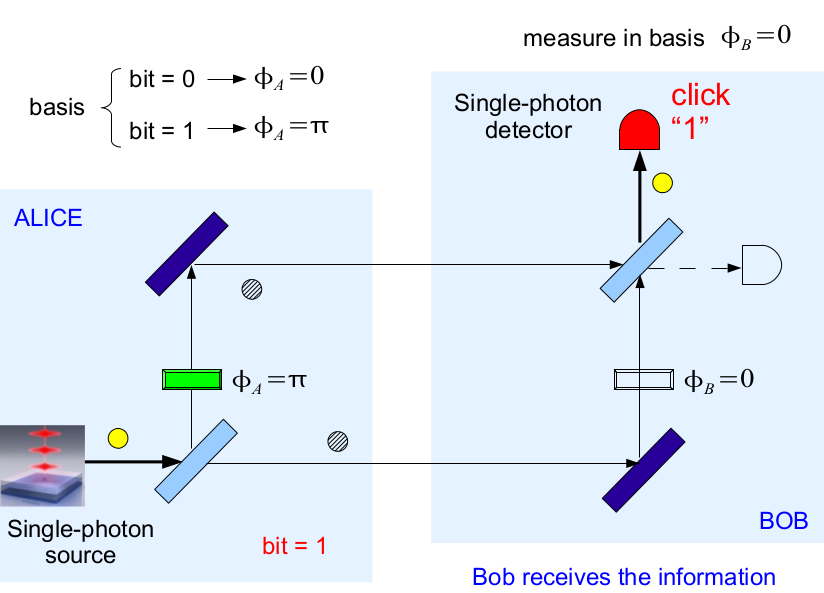
\includegraphics[scale=0.2]{ch3/image11}
	\captionof{figure}{ }
	\end{wrapfigure}
On cherche a déterminer l'état d'un photon. Pour y arriver, on va tout faire avec un McZehnder pour
le codage de l'information en phase. On se place dans la base
\begin{equation}
\left\{\begin{array}{ll}
\text{bit} = 0 &\to \Phi_A=0\\
\text{bit} = 1 &\to \Phi_A=\pi
\end{array}\right.
\end{equation}
Alice va utiliser une phase de $0$ ou $\pi$ si elle désire un $0$ ou $1$. Alice veut envoyer un zéro
et choisi alors $\Phi_A=0$. Si Bob mesure dans la base $\Phi_B=0$, il va avoir un clic '0' (il ne met pas de phase de son côté). Si Alice veut transmettre $1$, elle va utiliser $\Phi_A=\pi$. Si Bob mesure
dans la base $\Phi_B=0$ il aura un clic '1'. Dans les deux cas précédent, Bob reçoit l'information.\\

Si maintenant Alice envoie '0' ($\Phi_A=0$) et que Bob choisi de mesurer dans l'autre base
$\Phi_B=\pi/2$, il a 50\% de chance de clic '0' ou clic '1'. Le résultat est identique si Alice 
envoie '1' ($\Phi_A=\pi$). Dans les deux cas, Bob observe un bit aléatoire et n'a aucune information :
c'est parce qu'il a choisi la mauvaise base. \\

Troisième situation, Alice utilise maintenant la base
\begin{equation}
\left\{\begin{array}{ll}
\text{bit} = 0 &\to \Phi_A=\pi/2\\
\text{bit} = 1 &\to \Phi_A=3\pi/2
\end{array}\right.
\end{equation}
Si Alice envoie '0' ou '1' et que Bob utilise la base $\Phi_B=\pi/2$, il reçoit l'information dans
les deux cas car il est dans la bonne base. Si par contre Bob chance de base $\Phi_B=0$, il a de nouveau un bit aléatoire peu importe ce qu'envoie Alice. Il n'a pas d'information : il a choisi la mauvaise
base.\\

Ceci nous montre comment implémenter le "choix de base" présenté précédemment. Mais ce protocole
n'est pas pratique, car il nécessite l'existence d'un interféromètre qui peut être long d'une centaine
de kilomètres. Comment éviter l'interféromètre?


\subsection{Implémentation optique (multiplexage temporel)}
	\begin{wrapfigure}[7]{l}{6cm}
	\vspace{-5mm}
	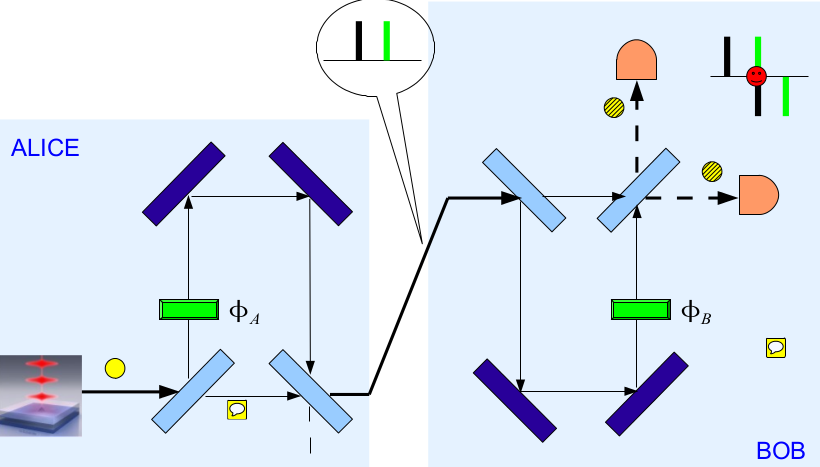
\includegraphics[scale=0.2]{ch3/image12}
	\captionof{figure}{ }
	\end{wrapfigure}
Pour l'éviter, on va multiplexer : on a maintenant à disposition deux petits interféromètres. Le
chemin peut être plus petit en fonction du bras emprunté et il en résulte un délai temporel. Le 
trait vert supérieur correspond à celui qui passe dans $\Phi_A$ tandis que le trait vers inférieur
celui que passe dans $\Phi_B$. Ils arrivent en retard, alors que le trait noir correspond au 
chemin "court" (arrive avant). 

\newpage
\subsection{Implémentation optique (codage en phase)}
	\begin{wrapfigure}[11]{l}{6cm}
	\vspace{-5mm}
	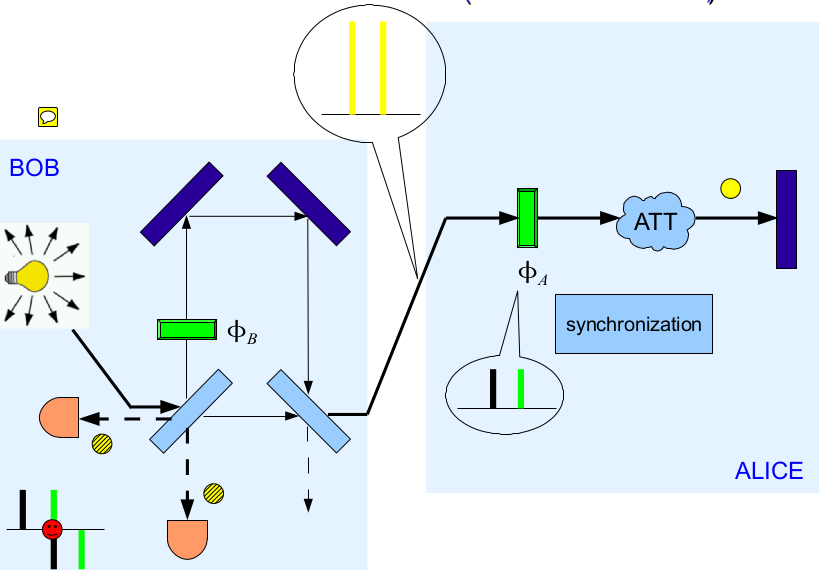
\includegraphics[scale=0.2]{ch3/image13}
	\captionof{figure}{ }
	\end{wrapfigure}
Il est possible de faire mieux et n'avoir qu'un seul interféromètre. Bob envoie une impulsion
lumineuse, pas du tout quantique, qui se propage dans l'interféromètre. Il en ressort deux 
impulsions : une en avance et une en retard (les deux jaunes). On les atténue (ATT) pour n'avoir
qu'un seul photon et on les renvoie du côté de Bob. Avant de les renvoyer, on va imposer une
phase différente aux deux photons (par synchronisation via l'électronique rapide). Par exemple, 
pas de phase sur un photon (photon noir) et une phase sur l'autre (photon vert) : on reconstruit 
ainsi les deux photons du premier interféromètre du cas précédent. Une fois chez Alice, tout se passe comme au précédent montage. Tout est identique, mais avec un interféromètre de moins. Voir 
\textit{slide 50} pour l'implémentation réelle (et commentaires).


\iffalse


\fi